%!TEX root = ../template.tex
%%%%%%%%%%%%%%%%%%%%%%%%%%%%%%%%%%%%%%%%%%%%%%%%%%%%%%%%%%%%%%%%%%%%
%% chapter4.tex
%% NOVA thesis document file
%%
%% Chapter with lots of dummy text
%%%%%%%%%%%%%%%%%%%%%%%%%%%%%%%%%%%%%%%%%%%%%%%%%%%%%%%%%%%%%%%%%%%%
\chapter{Planning} \label{cha:planning}

In this Chapter we begin by defining the system model and the intuition for the proposed solution followed by defining a set of metrics to evaluate it. In the last section we present the work plan for the remaining of the thesis. 

As previously mentioned, the challenge we propose to address is the creation of a large-scale decentralized management and monitoring infrastructure tailored for heterogenous edge devices. This infrastructure may be used to track the state of applications (for load balancing), discover nearby devices to offload tasks, or find a set of devices to deploy a new application in a strategic location, enabling in the future the autonomic management of edge-enabled applications.

\section{System Model}

As defined in section~\ref{sec:edge_computing}, the edge environment is composed by devices classified in levels ranging from [0-7]. From this classification, we outline two major categories:  

\textbf{Stable devices} consist of devices ranging from levels [0-5] in the taxonomy. We consider devices in these levels ``stable'' because they are usually connected across a wired medium (except in the case of laptops), which makes their connections more stable, and have enough computational capacity to perform monitoring and management tasks. 

\textbf{Unstable devices} are comprised by devices in levels 6 and 7. In the case of mobile devices (level 6), we consider them unstable due to their low computational power and the fact that their physical location may change rapidly, which may lead to topology mismatch. Furthermore, both devices in levels 6 and 7 are connected across a wireless medium, raising a large number of concerns that are outside the scope of this work.

Following, we have applications and, in the context of this thesis, we will only consider the management of \textbf{edge-enabled applications} running on containers. We consider these as applications which are decomposable into  multiple independent components and may be hosted in a single container. These applications may also function as a \textit{monolithic} applications, or alternatively have components hosted by containers scattered throughout the system.

Consequently, we define a set of operations which are critical for this type of applications: \textit{offloading} and \textit{migrating}. Offloading consists in delegating the task of hosting an application subcomponent to another device, whereas migrating means transferring a component (or multiple components) of the application to another device in the system. These two operations enable load-balancing through offloading tasks, scaling up or down depending on the computational capabilities of the device, and allow applications to improve their latency. 


During the execution of our solution, we assume that there is at most 1 simultaneous unexpected failure across the data centers belonging to the system. In addition, we assume that paths between any two nodes in the system have the same chance of failure regardless of the administrative domains they belong to.

%%%%%%%%%%%%%%%%%%%%%%%%%%%%%%%%%%%%%%%%%%%%%%%%%%%%%%%%%%%%%%%%%%
\section{Proposed Solution}
\label{cha:proposed_sol}

%As previously mentioned, the challenge we propose to address is to create a large-scale decentralized management and monitoring infrastructure tailored for heterogenous edge devices, which in turn may be used to track the status of applications, discover nearby devices to offload tasks, or find devices to deploy a set of services given certain constraints. 

\begin{figure}
    \centering
    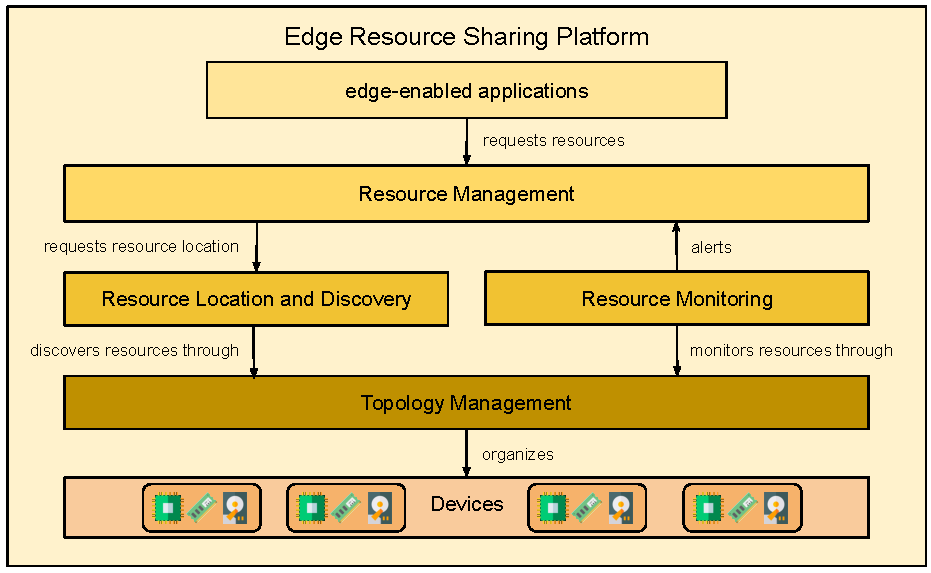
\includegraphics[width=0.9\linewidth]{Figures/proposed_architecture_detailed.pdf}
    \caption{High-level architecture of the proposed resource sharing platform}
    \label{fig:proposed_architecture_detailed}
\end{figure}

In the Figure \ref{fig:proposed_architecture_detailed}, we illustrate the proposed architecture of the solution we intend to design, which is composed of four co-dependent mechanisms exercised by every participant of the system.

At the bottom, we have \textbf{topology management}, whose responsibilities consist of: (1) ensuring that devices belonging to the overlay remain connected at all times; (2) materializing a hierarchical topology inspired on the capabilities of devices composing the system; (3) assuring that devices have at least one non-faulty device connected to it; (4) detecting failures of the participating nodes. This mechanism, inspired in works such as Astrolabe \cite{Renesse2003}, enables the correct behavior of the remaining components.

Following, we have \textbf{resource monitoring}, the objectives of this mechanism consist of: (1) collecting metrics about the containers hosting the applicational components; (2) aggregating the collected data in a decentralized manner; (3) deciding whether an application component hosted on certain device is not performing according to the established performance criteria; (4) alerting the resource management mechanism about failures in the containers and components performing sub-optimally.

The \textbf{resource management} mechanism handles the alerts emitted by the resource monitoring mechanism and, depending on the alert, immediately relocates application components to ensure they remain functional. As previously mentioned, scheduling optimal deployment configurations for application components is out of the scope of our work, given that it is an entire research topic on its own. With this in mind, our architecture will be tailored to accommodate an additional layer which performs resource scheduling. We envision this layer as an edge-enabled application, composed by multiple components, that will employ decentralized scheduling algorithms to determine the aforementioned optimal deployments.

%\todo{dizer deployment scheduling e depois chamar de resource scheduling é confuso. não está claro sobre qual é a diferença, ou que estás a falar da mesma coisa sequer. talvez meter entre () o resource scheduling quando falas da cena de deployment e mencionares que é um layer a cima do que estás a fazer. e quando te queres referir entao a esse layer, podes dizer accommodate to the/this/aforementioned upper layer}

To enable this, the resource management mechanism will provide two operations: a subscription operation which enables the resource scheduling mechanism to be notified whenever an application component changes its location due to the alerts or failures, and a operation for querying available resources and issuing deployment configurations. 

Lastly, we have the \textbf{resource location and discovery} mechanism. This mechanism will offer multiple search strategies which, in turn, will be employed by the resource management layer to replace failed components or to satisfy queries arising from the resource scheduling mechanism.

\section{Evaluation}  

In order to evaluate our work, we will employ a real-world scenario composed by devices ranging across the different levels of capacity and availability. The devices composing the test scenario consist of: devices in Cloud Environments (e.g. AWS or Azure), devices in the Grid5000 cluster and around 20 Raspberry Pis.

%In order to evaluate the implemented solution, and the advantages and disadvantages of the decentralized hierarchical model, 
We intend to develop two simple solutions 
%which are representative...
that will be representative of common architectures of monitoring systems. The first and most popular approach consists of a centralized controller for tracking and managing the state of devices and components running on them. %while the second approach...
On the other hand, the second approach consists of a flat decentralized model where peers are not organized into a hierarchical topology, 
%which means that...
meaning that all nodes in the system handle similar amounts of monitoring information. These simple solutions will serve as a baseline for our's.
%our solution.

In order to compare topologies, we define a set of system and applicational-related metrics. \textbf{System metrics} consist of the usage of system resources such as cpu, memory and bandwidth in each node of the system, followed by the number of required control messages to maintain the overlay.

\textbf{Application metrics} are related to the monitoring infrastructure running atop the overlay. The first metric to consider is \textit{cost}, that consists in the relation between the number of messages sent and the value of the information. 
%...,following, we have \textit{information freshness}, which consists in the timeliness of the information each node has of the system, and finally, \textit{information precision}, which represents the difference between the obtained monitoring data and the real status of the device / applications running on it. 
Following, we have \textit{information freshness}, that tracks the timeliness of the information each node has of the system, and, finally, \textit{information precision}, which represents the difference between the obtained monitoring data and the real status of the device / applications running on it. 


\section{Scheduling}

In this section we outline the identified tasks and the proposed work plan for the remaining of this thesis. 

\begin{enumerate}
    \item \textbf{Topology Management} (2/3/2020 - 4/4/2020)
    
    \begin{enumerate}
        \item Devise and develop the overlay algorithm which establishes the hierarchical topology (2/3/2020 - 31/3/2020)
        \item Validate the devised algorithm (21/3/2020 - 4/4/2020)
    \end{enumerate}
    
    \item \textbf{Resource Monitoring} (2/4/2020 - 23/5/2020)
    
    \begin{enumerate}
        \item Define the metrics to collect, and devise or adapt a monitoring probe which extracts these metrics from deployed components (2/4/2020 - 8/4/2020)
        \item Implement an adapt aggregation techniques for these metrics based on the overlay structure (10/4/2020 - 1/5/2020)
        \item Create or adapt an alerting solution which analyzes the aggregation results, detects anomalies on running components (e.g., sub-optimal performance) and emits alerts (1/5/2020 - 14/5/2020)
        \item Test the resource monitoring mechanism (26/4/2020 - 23/5/2020)
    \end{enumerate}
    
    \item \textbf{Resource Location and Discovery} (22/5/2020 - 6/10/2020)
    
    \begin{enumerate}
        \item Implement search algorithms which serve as tools for finding certain resources in the system (22/5/2020 - 7/6/2020)
        \item Test the implemented search solutions (31/5/2020 - 10/6/2020)
    \end{enumerate}
    
    \item \textbf{Resource Management} (7/6/2020 - 3/7/2020)
    
    \begin{enumerate}
        \item Implement the handlers for the alerts emitted by the monitoring mechanism (7/6/2020 - 21/6/2020)
        \item Implement subscription operations which, in turn, will be employed by the aforementioned resource scheduler (21/6/2020 - 30/6/2020)
        \item Test the resource management mechanism (27/6/2020 - 3/7/2020)
    \end{enumerate}

    \item \textbf{Evaluation} (1/7/2020 - 15/8/2020)
    
    \begin{enumerate}
        \item Develop the centralized and flat solutions to serve as baseline for evaluating the performance of the system (1/7/2020 - 13/7/2020)
        \item Develop simple mock-ups of edge-enabled applications (14/7/2020 - 21/7/2020)
        \item Perform an experimental assessment of the solution in a realistic test bed, and compare the performance between the developed system and the baseline solutions (22/7/2020 - 15/8/2020)
    \end{enumerate}

    \item \textbf{Thesis document} (1/7/2020 - 23/9/2020)
    
    \begin{enumerate}
        \item Review related work (1/7/2020 - 31/7/2020)
        \item Writing the document (3/3/2020 - 23/9/2020)
        \item Reviewing the written document (3/9/2020 - 23/9/2020)
    \end{enumerate}
    
\end{enumerate}


\begin{figure}[hbpt]
    \centering
    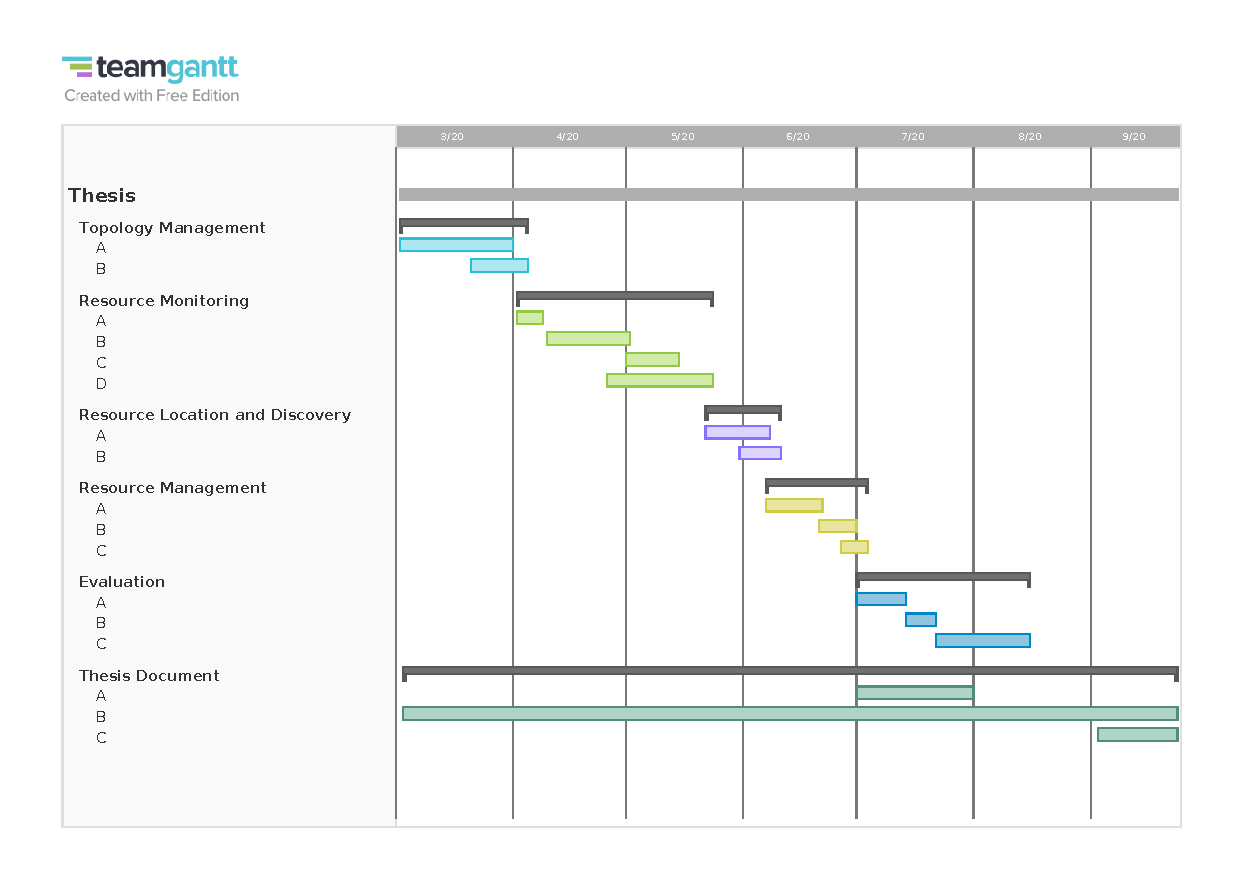
\includegraphics[width=0.95\linewidth]{Figures/gantt_chart.pdf}
    \caption{Gantt chart illustrating the work plan}
    \label{fig:gantt_chart}
\end{figure}
